\phantomsection
\numberedsection{RF4.1 Crear categoría}

\subsection*{Descripción}
Permite a los usuarios definir nuevas categorías para poder relacionarlas como etiquetas para los productos y facilitar la organización de forma personalizada.\par
\vspace{0.15cm}

\textbf{Pre-condición}\par
El usuario debe de tener la sesión iniciada en Mini PIM. \par
\vspace{0.15cm}

\textbf{Post-condición}
\begin{itemize}
    \item Caso de éxito: La categoría es creada correctamente, se muestra en la lista de categorías con el nombre ingresado y el contador de productos asociado inicia en cero.
    \item Caso mínimo: El sistema notifica al usuario el resultado de la acción de crear categoría: exitosa o fallida.
\end{itemize}

\textbf{Prioridad: }
Media
\vspace{0.15cm}

\textbf{Autor: }
Janine Bernadeth Olegario Laguit\par
\vspace{0.15cm}

\textbf{Control de cambios: } Versión 1: Definición del caso de uso

\numberedsubsection{Escenario principal}
\begin{enumerate}
    \item El usuario accede a la sección de gestión de categorías.
    \item El sistema muestra la lista de categorías existentes y la opción para crear una nueva.
    \item El usuario selecciona la opción para crear una nueva categoría.
    \item El sistema verifica el número total de categorías creadas por el usuario y compara el número de categorías creadas con el límite establecido por el plan de suscripción del usuario.
    \item El sistema muestra el menú de creación de categoría.
    \item El usuario ingresa el nombre deseado y confirma la creación de la categoría.
    \item El sistema verifica que el nombre de la categoría no esté vacío.
    \item El sistema crea la nueva categoría y actualiza la lista de categorías para incluirla.
    \item El usuario visualiza la nueva categoría en la lista, con el nombre ingresado y un contador de productos asociados que empieza en cero.
\end{enumerate}

\numberedsubsection{Escenarios alternativos}
\begin{description}

    \item[3.a] El sistema muestra un mensaje de error indicando que se ha alcanzado el límite de categorías permitido.
    \begin{enumerate}
        \item[3.a.1] El sistema no permite crear categorías adicionales hasta que se elimine una de las ya existentes o se amplíe el plan de suscripción.
    \end{enumerate}

    \item[5.a] El usuario cancela la acción de crear una categoría nueva seleccionando la opción que cierra el menú.
    \begin{enumerate}
        \item[5.a.1] El sistema regresa a la sección de gestión de categorías de los datos.
    \end{enumerate}

    \item[7.a] El sistema detecta que el nombre de la categoría está vacío.
    \begin{enumerate}
        \item[7.a.1] El sistema muestra un mensaje de error solicitando un nombre válido.
        \item[7.a.2] El sistema devuelve al usuario a la pestaña de gestión de categorías.
    \end{enumerate}
\end{description}

\numberedsubsection{Casos de Prueba}
\underline{Escenario: Principal}\par
\vspace{0.15cm}
\textbf{Dado} que he iniciado sesión con mi cuenta de usuario correspondiente\par
\textbf{Y} estoy en el apartado de Categorías\par
\textbf{Cuando} selecciono la opción de “Añadir categoría”\par
\textbf{E} introduzco correctamente el nombre de la categoría que deseo crear\par
\textbf{Y} selecciono “Confirmar” para guardar los datos\par
\textbf{Entonces} el sistema almacena la información de la nueva categoría en la base de datos del Mini PIM\par
\textbf{Y} actualiza la lista de categorías con la nueva categoría creada\par
\textbf{Y} muestra el apartado de Categorías con todas las categorías almacenadas, incluyendo la nueva con un contador de productos en cero.\par

\vspace{0.20cm}



\underline{Escenario: Alternativo 3.a}\par
\vspace{0.15cm}

\textbf{Dado} que he iniciado sesión con mi cuenta de usuario correspondiente\par
\textbf{Y} estoy en el apartado de Categorías\par
\textbf{Cuando} selecciono la opción de “Añadir categoría”\par
\textbf{Y} el sistema verifica el número de categorías creadas y el límite de categorías de mi plan de suscripción\par
\textbf{Entonces} el sistema me notifica que he alcanzado el límite de categorías permitido por mi plan\par
\textbf{Y} no me permite crear más categorías hasta que elimine una de las ya existentes o se amplíe el plan de suscripción.\par
\vspace{0.20cm}

\underline{Escenario: Alternativo 5.a}\par
\vspace{0.15cm}

\textbf{Dado} que he iniciado sesión con mi cuenta de usuario correspondiente\par
\textbf{Y} estoy en el apartado de Categorías\par
\textbf{Cuando} selecciono la opción de “Añadir categoría”\par
\textbf{Y} selecciono la opción de cancelar o cerrar el menú de creación sin ingresar ningún nombre\par
\textbf{Entonces} el sistema regresa a la sección de gestión de categorías\par
\textbf{Y} muestra el apartado de Categorías sin ningún cambio.\par

\vspace{0.20cm}

\underline{Escenario: Alternativo 7.a}\par
\vspace{0.15cm}

\textbf{Dado} que he iniciado sesión con mi cuenta de usuario correspondiente\par
\textbf{Y} estoy en el apartado de Categorías
\textbf{Cuando} selecciono la opción de “Añadir categoría”\par
\textbf{Y} dejo el campo de nombre de la categoría vacío\par
\textbf{Entonces} el sistema me notifica que el campo de nombre no puede estar vacío\par
\textbf{Y} muestra un mensaje de error y me devuelve al apartado de categorías sin ningún cambio.\par

\vspace{0.20cm}

\numberedsubsection{Bocetos}
\begin{figure}[H]
    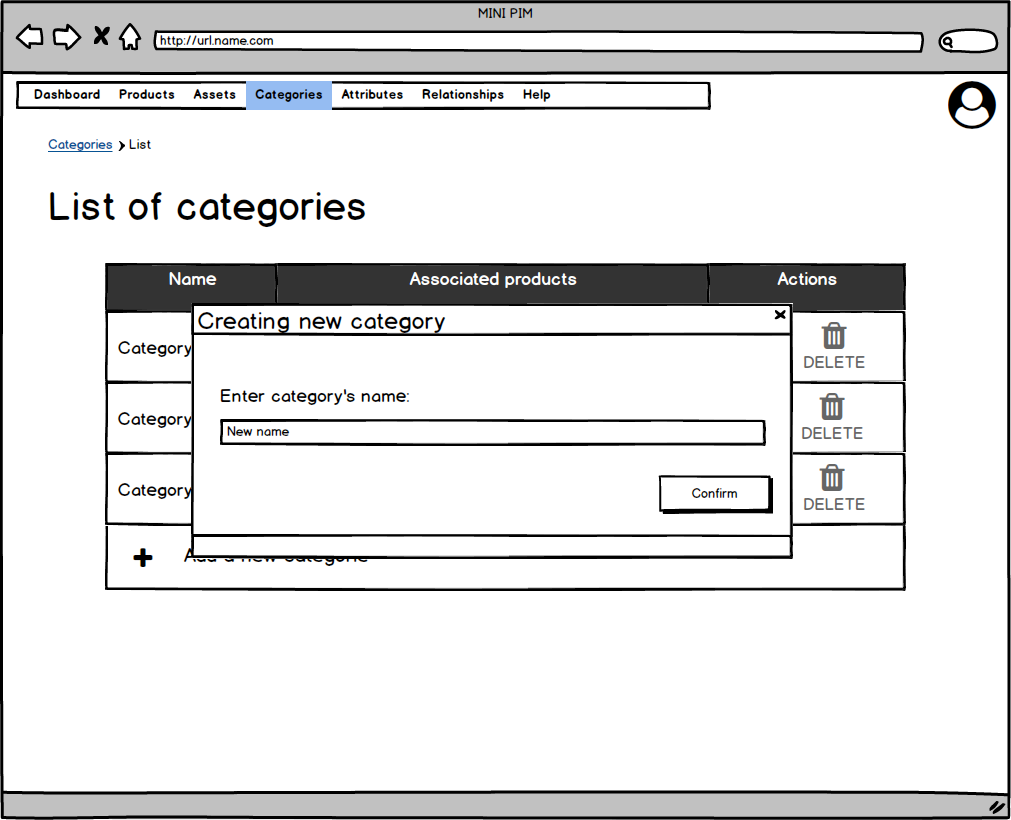
\includegraphics[width=1\linewidth]{mockups/RF4.1_1.png}
    \caption{Creación de categoría}
   \end{figure}
\vspace{1.0cm}

\begin{figure}[H]
    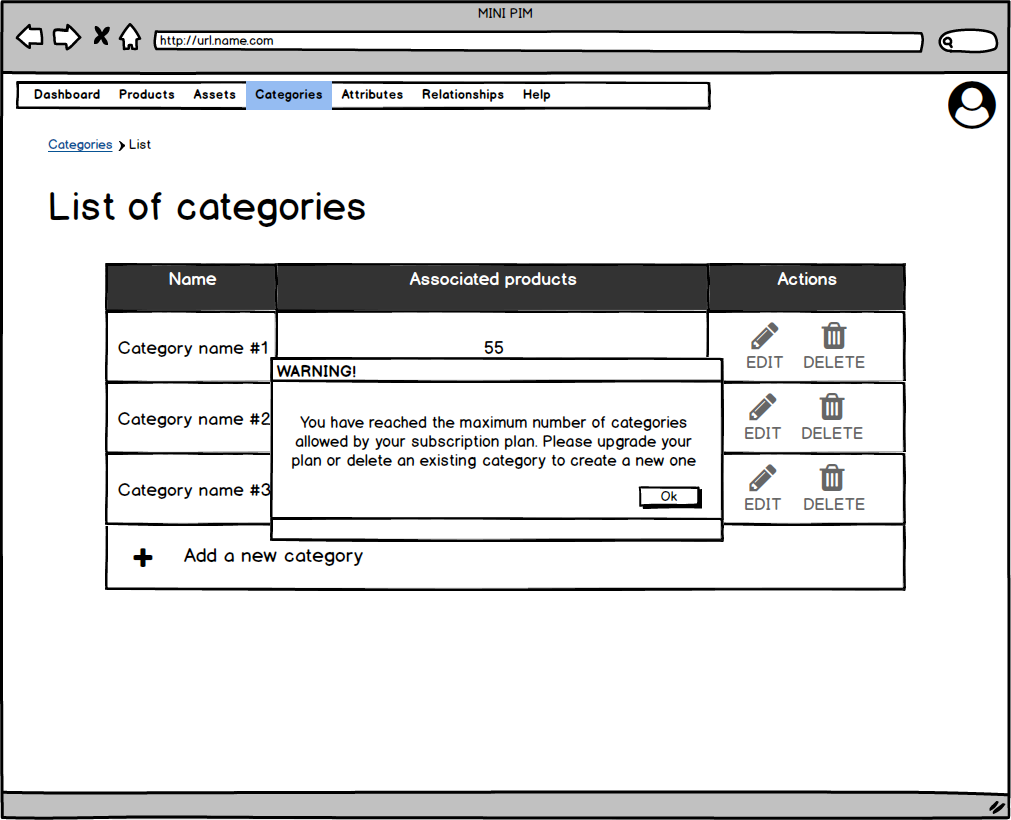
\includegraphics[width=1\linewidth]{mockups/RF4.1_2.png}
    \caption{Error por llegar al máximo de categorías}
   \end{figure}
\vspace{1.0cm}

\numberedsection{RF4.2 Visualizar categoría}

\subsection*{Descripción}
Permite a los usuarios visualizar una lista de categorías creadas en el sistema, incluyendo su nombre y el número de productos asociados a cada una.\par
\vspace{0.15cm}

\textbf{Pre-condición}\par
El usuario ha iniciado sesión en el sistema y se encuentra en el apartado de Categorías. \par
\vspace{0.15cm}

\textbf{Post-condición}
\begin{itemize}
    \item Caso de éxito: El sistema muestra la lista de categorías junto con el nombre y número de productos asociados.
    \item Caso mínimo: El sistema notifica al usuario el resultado de la acción de visualización de categorías: exitosa o fallida.
\end{itemize}

\textbf{Prioridad: }
Media
\vspace{0.15cm}

\textbf{Autor: }
Janine Bernadeth Olegario Laguit\par
\vspace{0.15cm}

\textbf{Control de cambios: } Versión 1: Definición del caso de uso

\numberedsubsection{Escenario principal}
\begin{enumerate}
    \item El usuario accede a la sección de gestión de categorías.
    \item El sistema muestra la lista de categorías existentes, incluyendo su nombre y el número de productos asociados.
\end{enumerate}

\numberedsubsection{Escenarios alternativos}
\begin{description}
    \item[2.a.] El sistema detecta que no existen categorías.
    \begin{enumerate}
        \item[2.a.1] El sistema muestra una lista vacía, con la opción de crear categorías nuevas.
    \end{enumerate}

\end{description}

\numberedsubsection{Casos de Prueba}
\underline{Escenario: Principal}\par
\vspace{0.15cm}

\textbf{Dado} que he iniciado sesión con mi cuenta de usuario correspondiente\par
\textbf{Y} estoy en el apartado de Categorías\par
\textbf{Entonces} el sistema muestra la lista de categorías existentes\par
\textbf{Y} cada categoría se visualiza junto a su nombre y el número de productos asociados.\par


\vspace{0.20cm}

\underline{Escenario: Alternativo 2.a}\par
\vspace{0.15cm}

\textbf{Dado} que he iniciado sesión con mi cuenta de usuario correspondiente\par
\textbf{Y} estoy en el apartado de Categorías\par
\textbf{Y} no existen categorías registradas en el sistema\par
\textbf{Entonces} el sistema muestra una lista vacía, con la opción de crear categorías nuevas.\par



\vspace{0.20cm}

\numberedsubsection{Bocetos}
\begin{figure}[H]
    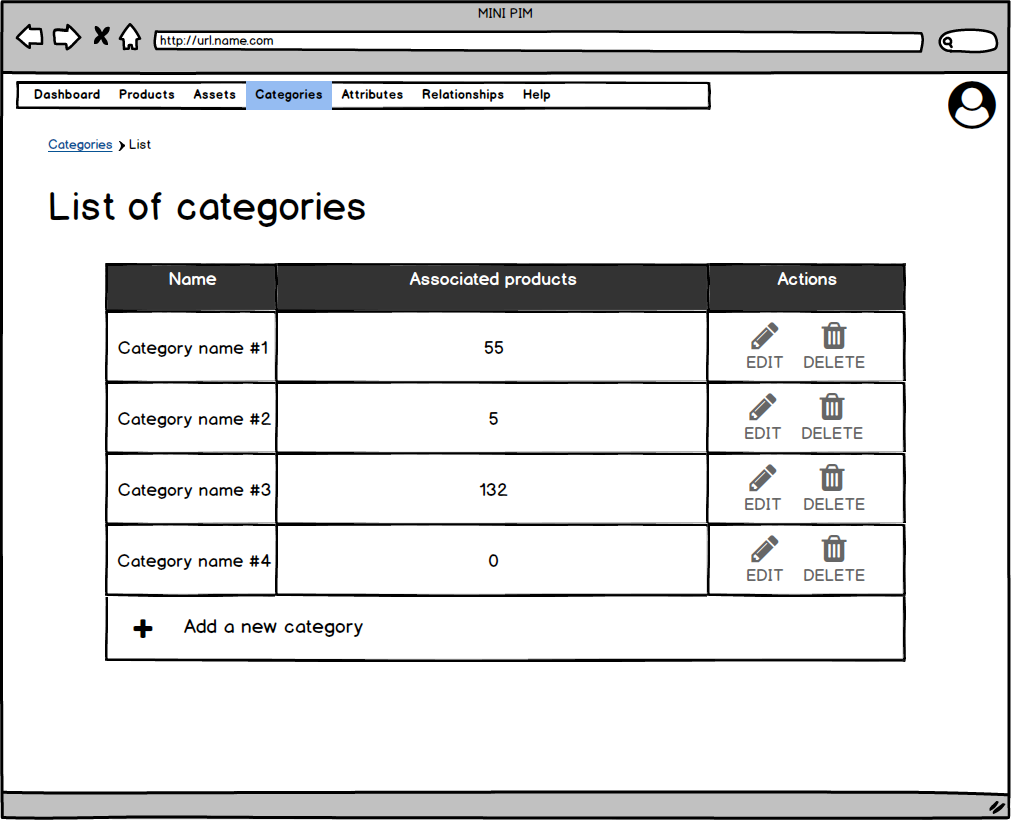
\includegraphics[width=1\linewidth]{mockups/RF4.2_1.png}
    \caption{Visualización de categorías}
   \end{figure}
\vspace{1.0cm}

\begin{figure}[H]
    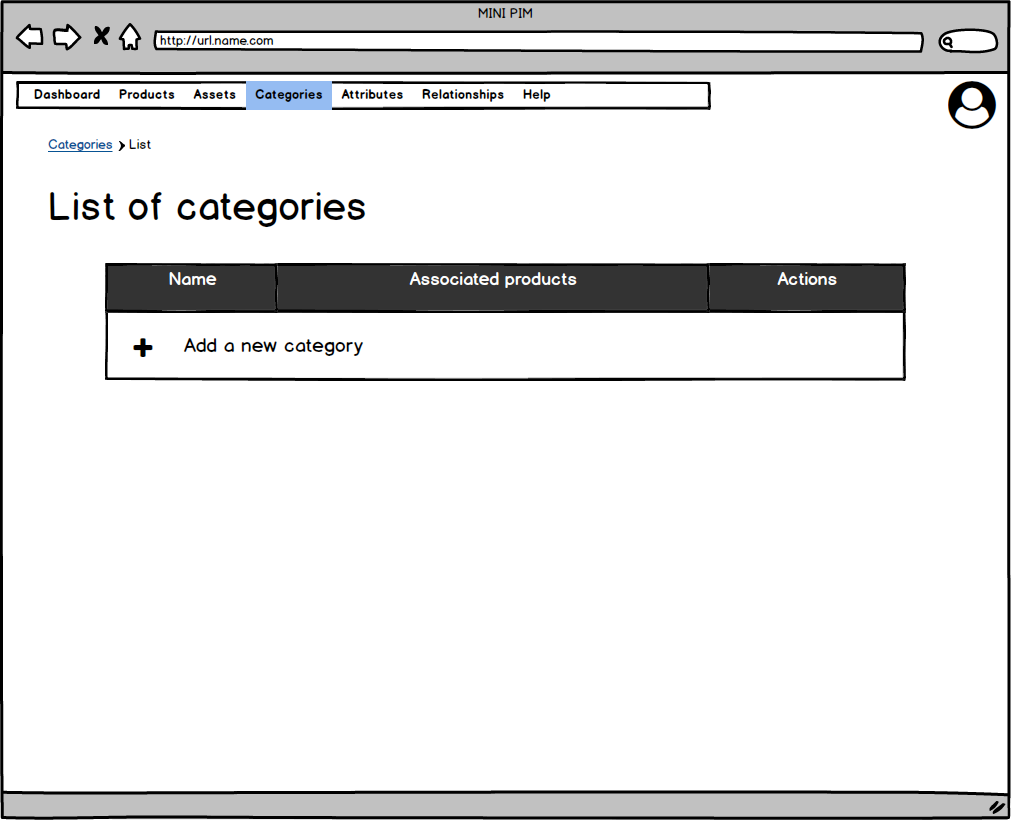
\includegraphics[width=1\linewidth]{mockups/RF4.2_2.png}
    \caption{Visualización de lista vacía}
   \end{figure}
\vspace{1.0cm}

\numberedsection{RF4.3 Editar categoría}

\subsection*{Descripción}
Permite a los usuarios modificar los datos de las categorías existentes.\par
\vspace{0.15cm}

\textbf{Pre-condición}\par
El usuario ha iniciado sesión en el sistema y se encuentra en el apartado de Gestión de Categorías. La categoría a editar debe existir en el sistema. \par
\vspace{0.15cm}

\textbf{Post-condición}
\begin{itemize}
    \item Caso de éxito: El sistema actualiza los datos de la categoría seleccionada y refleja los cambios en la lista de categorías.
    \item Caso mínimo: El sistema notifica al usuario el resultado de la acción de edición de la categoría: exitosa o fallida.
\end{itemize}

\textbf{Prioridad: }
Media
\vspace{0.15cm}

\textbf{Autor: }
Janine Bernadeth Olegario Laguit\par
\vspace{0.15cm}

\textbf{Control de cambios: } Versión 1: Definición del caso de uso

\numberedsubsection{Escenario principal}
\begin{enumerate}
    \item El usuario accede a la sección de gestión de categorías.
    \item El sistema muestra la lista de categorías existentes y la opción para editar una categoría.
    \item El usuario selecciona la opción de editar una categoría existente.
    \item El sistema presenta un menú con el nombre actual de la categoría.
    \item El usuario ingresa el nuevo nombre para la categoría.
    \item El usuario confirma la modificación del nombre.
    \item El sistema valida el nuevo nombre y actualiza la categoría en la base de datos.
    \item El sistema muestra un mensaje de éxito y refleja el nuevo nombre en la lista de categorías.
\end{enumerate}

\numberedsubsection{Escenarios alternativos}
\begin{description}
    \item[4.a] El usuario cancela la acción de editar la categoría seleccionada.
    \begin{enumerate}
        \item[4.a.1] El sistema regresa a la sección de gestión de categorías sin realizar ningún cambio.
    \end{enumerate}

    \item[6.a] El usuario deja el nombre de la categoría vacío.
    \begin{enumerate}
        \item[6.a.1] El sistema muestra un mensaje de error solicitando un nombre válido.
        \item[6.a.2] El usuario ingresa un nombre válido y confirma nuevamente.
    \end{enumerate}
\end{description}

\numberedsubsection{Casos de Prueba}
\underline{Escenario: Principal}\par
\vspace{0.15cm}

\textbf{Dado} que he iniciado sesión con mi cuenta de usuario correspondiente\par
\textbf{Y} estoy en el apartado de Categorías\par
\textbf{Cuando} selecciono la opción de editar una categoría existente\par
\textbf{Y} el sistema presenta un menú con el nombre actual de la categoría\par
\textbf{E} introduzco el nuevo nombre para la categoría\par
\textbf{Y} confirmo la modificación del nombre\par
\textbf{Entonces} el sistema valida el nuevo nombre\par
\textbf{Y} el sistema actualiza la categoría en la base de datos con el nuevo nombre\par
\textbf{Y} el sistema muestra un mensaje de éxito\par
\textbf{Y} refleja el nuevo nombre de la categoría en la lista de categorías.\par


\vspace{0.20cm}


\underline{Escenario: Alternativo 4.a}\par
\vspace{0.15cm}

\textbf{Dado} que he iniciado sesión con mi cuenta de usuario correspondiente\par
\textbf{Y} estoy en el apartado de Categorías\par
\textbf{Cuando} selecciono una categoría para editar\par
\textbf{Y} selecciono la opción de cancelar la acción de edición\par
\textbf{Entonces} el sistema regresa a la sección de gestión de categorías\par
\textbf{Y} muestra la lista de categorías sin realizar ningún cambio en la categoría seleccionada.\par

\underline{Escenario: Alternativo 6.a}\par
\vspace{0.15cm}

\textbf{Dado} que he iniciado sesión con mi cuenta de usuario correspondiente\par
\textbf{Y} estoy en el apartado de Categorías\par
\textbf{Cuando} selecciono una categoría para editar\par
\textbf{Y} dejo el campo de nombre de la categoría vacío\par
\textbf{Entonces} el sistema muestra un mensaje de error\par
\textbf{Y} me devuelve al gestor de categorías sin realizar ningún cambio.\par

\vspace{0.20cm}

\numberedsubsection{Bocetos}
\begin{figure}[H]
    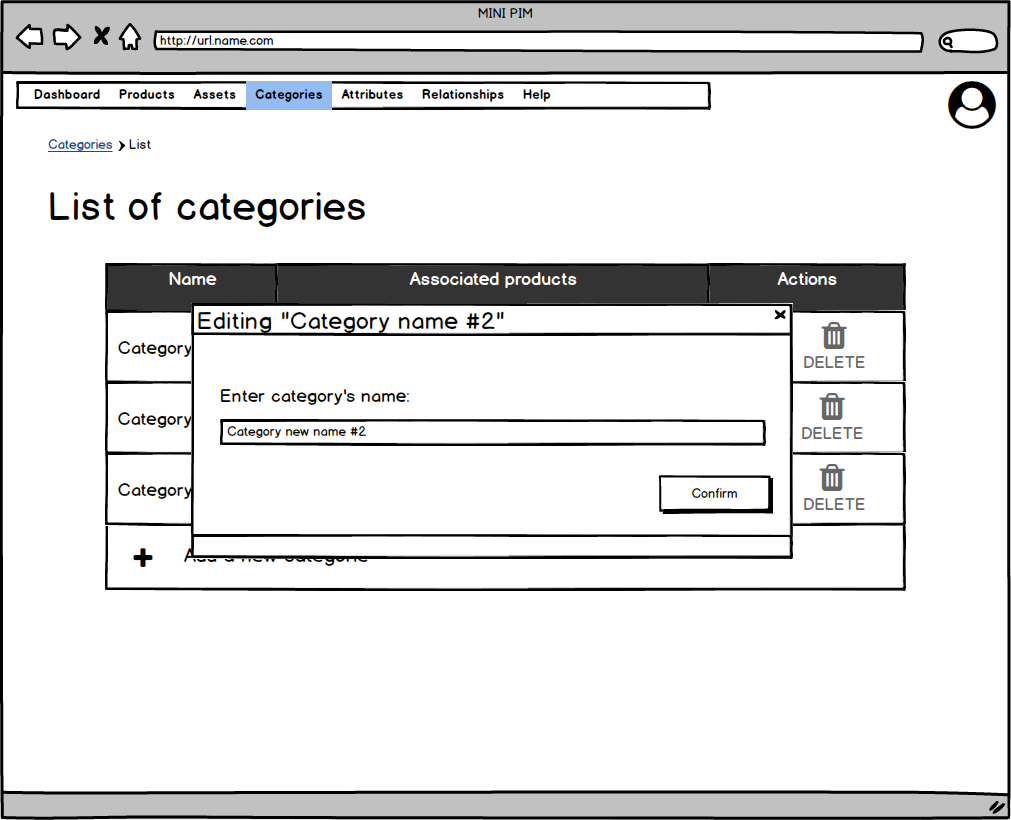
\includegraphics[width=1\linewidth]{mockups/RF4.3_1.png}
    \caption{Editar el nombre de categoría}
   \end{figure}
\vspace{1.0cm}

\begin{figure}[H]
    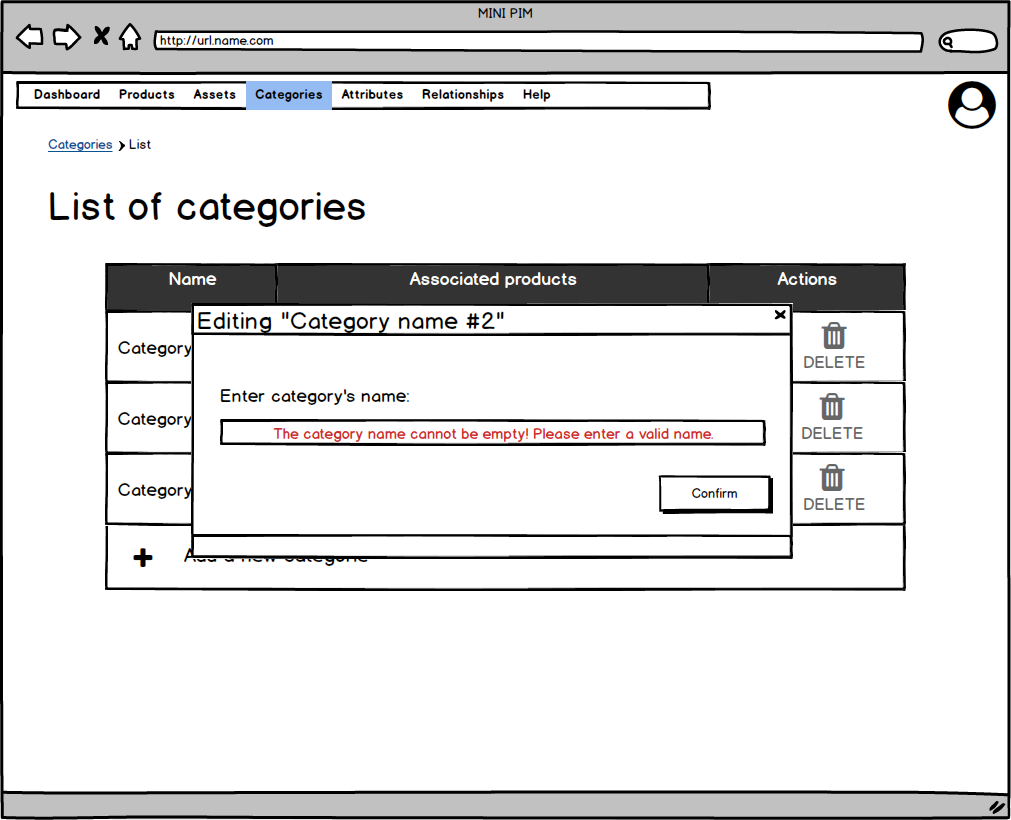
\includegraphics[width=1\linewidth]{mockups/RF4.3_2.png}
    \caption{Error por dejar el nombre vacío}
   \end{figure}
\vspace{1.0cm}

\numberedsection{RF4.4 Borrar categoría}

\subsection*{Descripción}
Permite a los usuarios eliminar una categoría existente en el sistema. La eliminación de una categoría solo será permitida si no está asociada a productos. \par
\vspace{0.15cm}

\textbf{Pre-condición}\par
El usuario debe tener la sesión iniciada en Mini PIM y tener acceso a la sección de gestión de categorías. La categoría a eliminar debe de existir en el sistema. \par
\vspace{0.15cm}

\textbf{Post-condición}
\begin{itemize}
    \item Caso de éxito: La categoría es eliminada correctamente, se elimina de la lista de categorías y se actualiza la base de datos.
    \item Caso mínimo: El sistema notifica al usuario el resultado de la acción de borrar categoría: exitosa o fallida.
\end{itemize}

\textbf{Prioridad: }
Media
\vspace{0.15cm}

\textbf{Autor: }
Janine Bernadeth Olegario Laguit\par
\vspace{0.15cm}

\textbf{Control de cambios: } Versión 1: Definición del caso de uso

\numberedsubsection{Escenario principal}
\begin{enumerate}
    \item El usuario accede a la sección de gestión de categorías.
    \item El sistema muestra la lista de categorías existentes
    \item El usuario selecciona la opción de eliminar una categoría
    \item El sistema muestra una ventana emergente de confirmación para la eliminación de la categoría
    \item El sistema verifica si la categoría está asociada a algún producto
    \item Si la categoría no está asociada a elementos críticos, el usuario confirma la eliminación
    \item El sistema elimina la categoría de la base de datos
    \item El sistema actualiza la lista de categorías, eliminando la categoría seleccionada
    \item El sistema muestra un mensaje de éxito indicando que la categoría ha sido eliminada correctamente
\end{enumerate}

\numberedsubsection{Escenarios alternativos}
\begin{description}
  
    \item[4.a] El usuario cancela la acción de eliminar la categoría seleccionada.
    \begin{enumerate}
        \item[4.a.1] El sistema regresa a la sección de gestión de categorías sin realizar ningún cambio.
    \end{enumerate}

     \item[6.a] La categoría seleccionada no puede ser eliminada por estar asociada a productos.
    \begin{enumerate}
        \item[6.a.1]  El sistema muestra un mensaje de error indicando que no se puede eliminar la categoría debido a que está asociada a algún producto.
        \item[6.a.2]  El sistema regresa a la sección de gestión de categorías.
    \end{enumerate}
\end{description}

\numberedsubsection{Casos de Prueba}
\underline{Escenario: Principal}\par
\vspace{0.15cm}

\textbf{Dado} que he iniciado sesión con mi cuenta de usuario correspondiente\par
\textbf{Y} estoy en el apartado de Categorías\par
\textbf{Cuando} selecciono la opción de Eliminar en una categoría\par
\textbf{Y} confirmo la eliminación de la categoría en la ventana emergente\par
\textbf{Entonces} el sistema elimina la categoría de la base de datos\par
\textbf{Y} actualiza la lista de categorías, removiendo la categoría eliminada\par
\textbf{Y} muestra un mensaje de éxito indicando que la categoría ha sido eliminada correctamente.\par




\vspace{0.20cm}

\underline{Escenario: Alternativo 4.a}\par
\vspace{0.15cm}

\textbf{Dado} que he iniciado sesión con mi cuenta de usuario correspondiente
\textbf{Y} estoy en el apartado de Categorías\par
\textbf{Cuando} selecciono la opción de Eliminar en una categoría\par
\textbf{Y} selecciono la opción de Cancelar en la ventana emergente de confirmación\par
\textbf{Entonces} el sistema regresa a la sección de gestión de categorías\par
\textbf{Y} muestra la lista de categorías sin realizar ningún cambio.\par


\vspace{0.20cm}

\underline{Escenario: Alternativo 6.a}\par
\vspace{0.15cm}

\textbf{Dado} que he iniciado sesión con mi cuenta de usuario correspondiente\par
\textbf{Y} estoy en el apartado de Categorías\par
\textbf{Cuando} selecciono la opción de Eliminar en una categoría\par
\textbf{Y} el sistema detecta que la categoría está asociada a algún producto\par
\textbf{Entonces} el sistema muestra un mensaje de error indicando que no se puede eliminar la categoría debido a su asociación con otros elementos importantes\par
\textbf{Y} el sistema me redirige a la sección de gestión de categorías\par


\vspace{0.20cm}

\numberedsubsection{Bocetos}
\begin{figure}[H]
    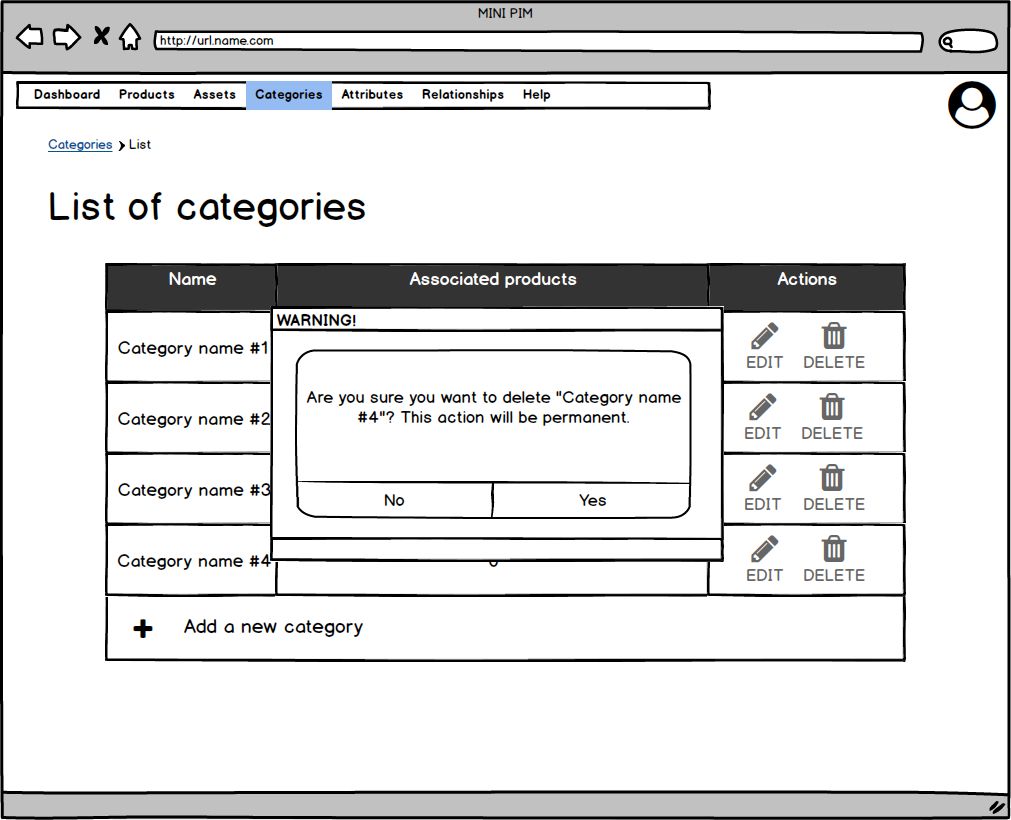
\includegraphics[width=1\linewidth]{mockups/RF4.4_1.png}
    \caption{Mensaje esperando confirmación para eliminar categoría}
   \end{figure}
\vspace{1.0cm}

\begin{figure}[H]
    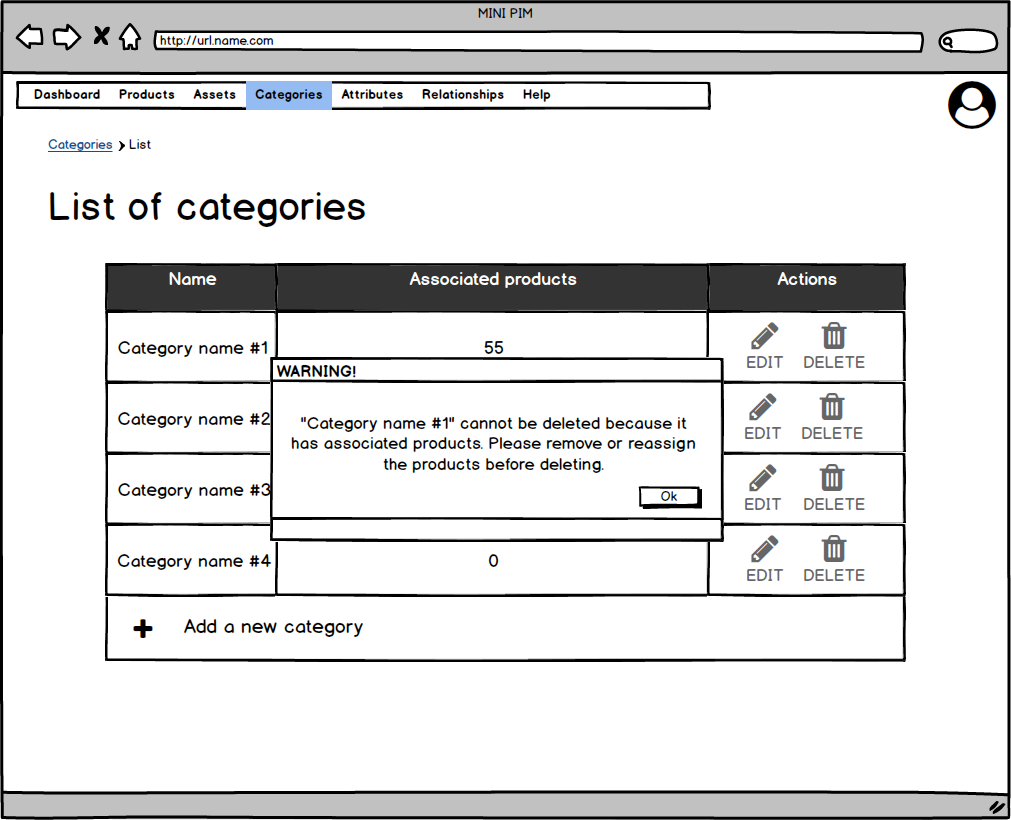
\includegraphics[width=1\linewidth]{mockups/RF4.4_2.png}
    \caption{Mensaje de error porque la categoría a borrar tiene productos asociados}
   \end{figure}
\vspace{1.0cm}

\newpage %Inicia en una nueva página otro caso de uso